\documentclass[12pt]{article}
\usepackage{a4wide}
\usepackage[utf8]{inputenc}
\usepackage[russian]{babel}
\usepackage[dvips]{graphicx, color}
\usepackage[section]{placeins}
\usepackage{epstopdf}
\usepackage{listings}
\usepackage{amsmath}
\usepackage{amsfonts}
\usepackage{amssymb}
\usepackage{textcomp}
\usepackage{amsthm}
\usepackage{tikz}
\usepackage{pgfplots}
\usepackage{titletoc}

\dottedcontents{section}[1.5em]{}{1em}{5pt}
\dottedcontents{subsection}[5.5em]{}{2.2em}{5pt}

\lstdefinelanguage{Scheme}{
  morekeywords=[1]{define, define-syntax, define-macro, lambda,
    define-stream, stream-lambda},
  morekeywords=[2]{begin, call-with-current-continuation, call/cc,
    call-with-input-file, call-with-output-file, case, cond,
    do, else, for-each, if,
    let*, let, let-syntax, letrec, letrec-syntax,
    let-values, let*-values,
    and, or, not, delay, force,
    quasiquote, quote, unquote, unquote-splicing,
    map, fold, syntax, syntax-rules, eval, environment, query,
    display, newline,list, apply, null?, car, cdr, for-each, 
make-vector, vector-length, vector-ref, vector-set!, eqv?, eq?, equal?, set!, 
define-record-type, fields, mutable, immutable, assert, parent, with-exception-handler,
  },
  morekeywords=[3]{import, export},
  alsoletter=?!-,
  alsodigit=\$\%&*+./:<=>@^_~,
  sensitive=false,
  morecomment=[l]{;},
  morecomment=[s]{/*}{*/},
  morestring=[b]",
  basicstyle=\small\ttfamily,
  keywordstyle=\bf\ttfamily\color[rgb]{0,.3,.7},
  commentstyle=\color[rgb]{0.133,0.545,0.133},
  stringstyle={\color[rgb]{0.75,0.49,0.07}},
  upquote=true,
  breaklines=true,
  breakatwhitespace=true,
  literate=*{`}{{`}}{1}
}

\begin{document}
\newcommand{\anonsection}[1]{\section*{#1}\addcontentsline{toc}{section}{#1}}

\renewcommand\appendixname{Приложение}
\makeatletter
\def\redeflsection{\def\l@section{\@dottedtocline{1}{1.5em}{7.8em}}}
\renewcommand\appendix{\par
\setcounter{section}{0}%
\setcounter{subsection}{0}%
\def\@chapapp{\appendixname}%
\addtocontents{toc}{\protect\redeflsection}
\def\thesection{\appendixname\hspace{0.2cm}\@arabic\c@section}}
\makeatother



\thispagestyle{empty}

\begin{center}
\ \vspace{-3cm}


\includegraphics[width=0.5\textwidth]{msu.eps}\\

{\scshape Московский государственный университет имени М.~В.~Ломоносова}\\
Факультет вычислительной математики и кибернетики\\
Кафедра системного программирования

\vfill

{\LARGE Отчёт по второму заданию}

\vspace{1cm}

{\Huge\bfseries Вариант №16: <<Выполнимость КНФ>>} \\

\end{center}

\vspace{1cm}

\begin{flushright}
  \large
  \textit{Задание выполнил студент 427 группы}\\
  Кольцов Михаил Андреевич

\end{flushright}

\vfill

\begin{center}
Москва, 2014
\end{center}

\pagebreak
\tableofcontents
\pagebreak

\newtheorem{definition} {Определение}
\newtheorem{option} {Свойство}
\newtheorem{theorem} {Теорема}


\section{Постановка задачи}
    Требуется написать программу на языке Scheme, которая по заданной  \textit{конъюнктивной нормальной форме} (далее~--- КНФ) определяет, является ли она выполнимой.
    При этом в решении должен использоваться \textit{генетический алгоритм} (описан в главе 3).

    Формально:

    \textbf{Литера}: переменная $x_i$ или отрицание переменной $\overline{x_i}$;

    \textbf{Дизъюнкция} $n$ литер $L_1, L_2, \ldots, L_n$: \space $L_1 \lor L_2 \lor \ldots \lor L_n$ (здесь $\lor$ -- опрератор логического ИЛИ);

    \textbf{КНФ} $n$ дизъюнкций $A_1, A_2, \ldots, A_n$: \space $A_1 \land A_2 \land \ldots \land A_n$ (здесь $\land$ -- опрератор логического И). Будем обозначать $Var(X)$ 
    множество всех литер КНФ $X$;

    \textbf{КНФ X выполнима} тогда и только тогда, когда $\exists v = (b_1, b_2, \ldots, b_{|Var(X)|}), b_i \in \{0, 1\},$ такое, что если в $X$ заменить $\forall x_i \in Var(X)$ на $b_i$, то полученное
    выражение будет истинно.

    В программу КНФ задаётся в виде списка списков. Все списки внутри большого списка рассматриваются как дизъюнкции, объединённые конъюнкцией. 
    В каждом списке-дизъюнкции элементами являются символы (например, $alpha$ или $x$) либо списки из двух элементов ($not$ символ), обозначающие отрицания.

    Например, выражение
    $$ (\overline{x_1}) \land (x_{10} \lor \overline{x_{11}} \lor x_{101}) $$
    будет представлено в виде списка (((not x1)) (x10 (not x11) x101)).

\pagebreak
\section{Генерация тестов}
    Чтобы проверить правильность функционирования программы, был подготовлен генератор тестов, который создаёт (в зависимости от параметров) тестовую КНФ, а также 
    заведомо правильный ответ для неё, а в случае выполнимости~--- ещё и одно из возможных решений.

    \subsection{Поддерживаемые параметры}
    \begin{enumerate}
        \item Количество дизъюнкций в КНФ (минимальное/максимальное);
        \item Количество литер в дизъюнкциях (минимальное/максимальное);
        \item Количество различных литер (минимальное/максимальное);
        \item Количество решений (минимальное/максимальное);
        \item Параметр \textit{амлпификации}.
    \end{enumerate}

    \subsection{Амплификация}
    Для того, чтобы вместе с тестами создавать возможные решения, использовался переборный алгоритм: для каждого $v = (b_1, b_2, \ldots, b_{|Var(X)|})$ проверяем истинность выражения. В случае
    истинности добавляем $v$ во множество ответов.

    Поскольку переборный алгоритм не справляется с решением задачи при большом числе переменных, мною был придуман способ увеличения тестового примера с сохранением знания обо всех 
    решениях, который я назвал \textbf{амплификация} (от англ. \textit{amplify}~--~<<усиливать>>). Суть способа в следующем. Пусть у нас имеется КНФ
    $$ X = A_1 \land A_2 \land \ldots \land A_n .$$
    Составим новую КНФ:
    $$ X_{amp} = X_1 \land X_2 \land \ldots \land X_{amp\_factor}$$
    $$ X_j = A_{1j} \land A_{2j} \land \ldots \land A_{nj}, $$
    где $A_{ij}$~--- дизнюнкция $A_i$, в которой каждя литера $t$ переименована в $t_{j}$.

    Заметим, что если известен ответ $$v = (b_1, b_2, \ldots, b_{|Var(X)|})$$ для $X$, то ответ для $X_{amp}$ представляет из себя $$v_{amp} = (b_{11}, b_{12}, \ldots, b_{1|Var(X)|},
    b_{21}, b_{22}, \ldots, b_{2|Var(X)|}, \ldots, b_{amp\_factor1}, \ldots, b_{amp\_factor|Var(X)|}),$$ где $b_{ij} = b_j$.

    Также зафиксируем соотношения между параметрами в исходном и амплифицированном выражениях:
    \begin{itemize}
        \item У $X$ есть $num$ решений $\rightarrow$ у $X_{amp}$ есть $num^{amp\_factor}$ решений.
        \item В $X$ присутствует $l$ различных литер $\rightarrow$ в $X_{amp}$ присутствует $l * amp\_factor$ различных литер.
    \end{itemize}

    \subsection{Тестовые данные}
    Таким образом, если сгенерировать <<маленький>> тест и приписать его самому к себе с переименованием переменных $amp\_factor$ раз, то получится тест со сколь угодно (в зависимости
    от величины $amp\_factor$) большим количество переменных, решений, дизъюнкций и литер.

    Параметры генерации тестовых случаев выбирались из следующих соображений:
    \begin{itemize}
        \item $\frac{s^{amp\_factor}}{2^{m * amp\_factor}} <= 10^{-9}$, где $s$~-- параметр \textit{количества решений}
            , $m$~-- параметр \textit{количества различных переменных}. Иными словами,
            решением должен являться не более чем каждый миллиардный случайно выбранный булев вектор.
        \item Параметры \textit{длины дизъюнкции} и \textit{количества дизъюнкций}
            выбирались так, чтобы генерация теста не занимала много времени. От этих параметров зависит количество решений (чем
            больше дизъюнкций, тем больше шанс сгенерировать неразрешимое противоречие $x_i \land \overline{x_i}$; а чем больше длина дизъюнкции, тем выше шанс получить
            подвыражение вида $x_i \lor \overline{x_i}$, которое автоматически делает истинным данную дизъюнкцию). Оптимальными я считаю
            значения $5 <=$ длина дизъюнкции $<= 7$ и $7 $ <= количество
            дизъюнкций $ <= 12$.
        \item \textit{Параметр амплификации} выбирался таким, чтобы итоговое количество переменных не превышало 100 (в целях более быстрого прогона тестов).
    \end{itemize}

    Решению подавались на вход как амплифицированные, так и неамплифицированные тесты.

    \subsection{Основные моменты реализации}

    В программе за генерацию тестов отвечает функция \textbf{generate-tests}. Значения параметров установлены в виде констант. Основные функции: \textit{gen-brace}
    (генерирует дизъюнкцию), \textit{gen-expr} (генерирует КНФ), \textit{amp-vars} и \textit{amp-expr} (амплифицируют КНФ и решение), а также \textit{gen-substitutions}
    (участвует в переборном решении). 
    
    Результат генерации возвращается функций \textit{output-loop} в виде списка тестов, где каждый тест~--- тройка <КНФ, есть решение?, одно из
    решений (или пустой список, если решения нет)>.


\pagebreak

    \section{Генетический алгоритм}
        Общая схема генетического алгоритма в программе состоит из \textit{итераций}, на каждой из которых происходит следующее:
        \begin{enumerate}
            \item Определённый процент особей из популяции претерпевает \textit{мутацию};
            \item Определённый процент особей из популяции \textit{скрещивается} друг с другом;
            \item Выбирается самый лучший (согласно \textit{оценочной функции}) представитель популяции. Если функция на нём принимает максимально возможное значение,
                то алгоритм завершается и выдаёт в качестве ответа этого представителя;
            \item В противном случае, часть особей погибает в процессе естественного \textit{отбора}, а алгоритм переходит к следующей итерации.
        \end{enumerate}

        Перед первой итерацией создаётся \textit{начальная популяция} случайным образом.

        \subsection{Описание особи}
        Каждая особь в популяции представляет из себя булев вектор $v_i = (b_1, b_2, \ldots, b_{|Var(X)|})$, где $X$~-- входная КНФ. Одна хромосома~-- одна из компонент этого вектора.

        \subsection{Описание оценочной функции}
        Пусть в тестовой КНФ $X$ содержится $n$ дизъюнкций $A_1, A_2, \ldots, A_n$. Обозначим за $A_j(v_i)$ выражение, полученное из $A_j$ заменой всех переменных на соответствующие
        им значения из $v_i$.
        Тогда функция $score$, оценивающая особь $v_i$ из популяции, задаётся следующим образом:
        $$ score(v_i) = \frac{|\{A_j | A_j(v_i) = true, j \in \overline{1..n}\}|}{n}.$$

        \subsection{Описание мутации и скрещивания}
        При мутации, особь $v_i$ инвертирует несколько своих случайно выбранных переменных.

        При скрещивании двух особей $v_i$ и $v_j$ происходит следующее. Сначала в качестве результата $child$ берётся $v_i$. Затем $\forall k \in \overline{1..n}$ 
        происходит замена $k$-го 
        элемента $child$ на $k$-ый элемент $v_j$. Если при такой замене оценочная функция становится больше, то в $child$ записывается $k$-й элемент из $v_j$. В противном
        случае $k$-е значение остаётся неизменным.

        \subsection{Описание способа отбора}
        Поддерживается инвариант: на начало каждой итерации в популяции должно быть заданное (зависящего от входной КНФ)
        количество особей. Для обеспечения этого инварианта в конце каждой итерации
        происходит отбрасывание самых худших (согласно оценочной функции) особей.

        \subsection{Критерий останова}
        Если на шаге 3 генетического алгоритма обнаруживается ответ, то алгоритм немедленно прекращает работу. В противном случае, по прошествии заданного числа итераций (зависящего
        от входной КНФ) алгоритм завершает работу с результатом <<решения нет>>.

        \subsection{Основные моменты реализации}
        Главная функция генетического алгоритма~-- \textbf{genetics-solver}. Внутри в виде переменных записаны параметры работы алгоритма (количество итераций, размер популяции,
        процент скрещиваемых на каждой итерации особей, процент мутирующих на каждой итерации особей, количество изменяемых хромосом в процессе мутации).
        Основные функции: \textit{breed-one-vs-one} (скрещивание двух особей), \textit{gen-mutate} (мутация особи),
        \textit{make-initial-population} (создание начальной популяции), \textit{genetics-iteration-loop}
        (цикл итераций генетического алгоритма).


\pagebreak

	\section{Визуализация}

        \subsection{Приближение текущего решения задачи к оптимальному}
        На каждой итерации генетического алгоритма снимаются два показания: наибольшее и наименьшее значение оценочной функции в текущей популяции. Эта информация собирается и 
        визуализируется в виде графика (см. рис. 1), который выводится после окончания работы алгоритма. Красной ломаной обозначается наибольшее значение оценочной функции, зелёной~-- наименьшее.
        Этот график позволяет оценить, насколько быстро решение подбирается к оптимальному. 

        Реализация этой части программы расположена в функции \textbf{check-test} в виде вывода графиков.

        \subsection{Найденное решение}
        Чтобы визуализировать найденное решение, я строю двудольный граф. В первой доле находятся дизъюнкции, во второй~-- переменные. Ребро проведено из каждой дизъюнкции
        в каждую переменную, которая в ней встречается. Если переменная имеет при подстановке в дизъюнкцию значение $True$, то ребро окрашено зелёным цветом, в противном случае~--
        синим. 

        После окончания работы алгоритма (в случае, если было найдено решение) появляется картинка (см. рис. 2), на которой изображается вышеописанный граф. Каждой вершине приписывается
        символьное описание (переменным~-- название и значение, дизъюнкциям~-- математическая запись). Благодаря цвету стрелок можно понять, насколько уникальными являются найденные
        значения переменных. Размер картинки выбирается в зависимости от входной КНФ, так что различные дизъюнкции визуально не <<наезжают>> друг на друга.

        Реализация этой части программы расположена в функции \textbf{draw-solution}. В ней происходит инициализация картинки, построение вершин графа, их соединение и раскраска
        рёбер. Используется много вспомогательных функций.


        \pagebreak
        \begin{figure}[b]
            \centering
            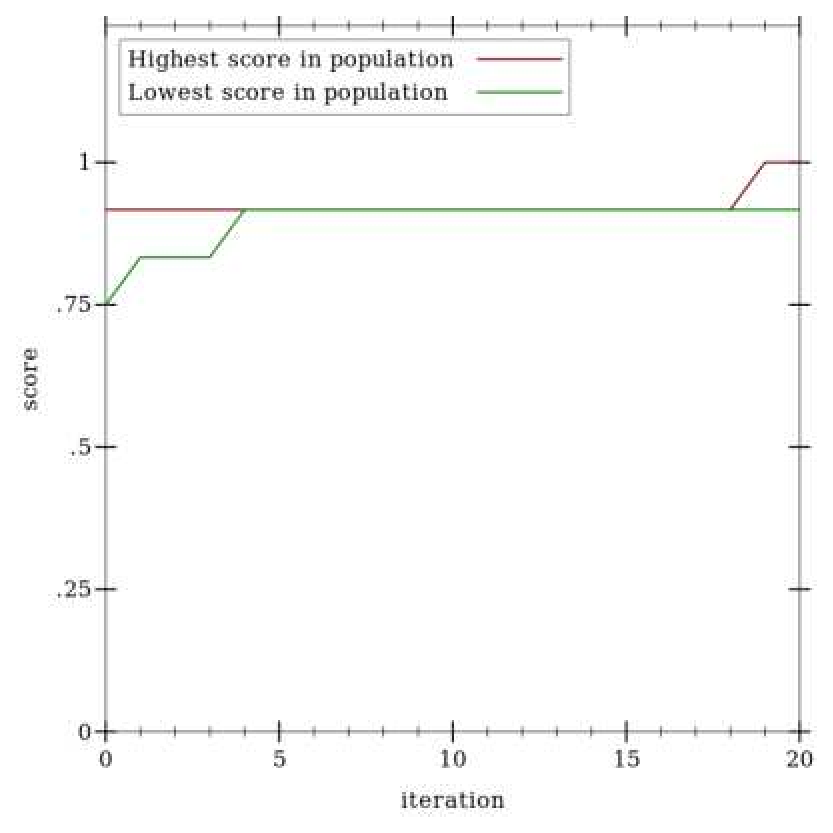
\includegraphics[scale=0.8]{plot.eps}
            \caption{Пример визуализации процесса приближения текущего решения к оптимальному}
            \includegraphics[scale = 0.7, trim = 1mm 1mm 1mm 10mm, clip]{graph.eps}
            \caption{Пример визуализации решения}
        \end{figure}

							
        \pagebreak

        \section{Результаты}

        \subsection{Неамплифицированные тесты}
        В данном тестовом случае решение работало верно более чем в 90\% запусков. По времени запуск одного теста занимает 
        меньше одной минуты. Причиной единичных неудач я вижу <<невезучесть>> рандомизации:
        видимо, иногда случайные мутации и скрещивания происходили исключительно непродуктивно. Впрочем, это случалось не так уж часто. 

        \subsection{Амплифицированные тесты}
        Для амплифицированных тестов успешность запусков программы составляет около 50\%. Тесты, в которых правильным ответом является <<решения нет>>, программа проходит безошибочно.
        Там, где решение есть, часто происходит <<застревание>> прогресса со значением функции около $0.9$. Я думаю, что реализовал алгоритм слишком неоптимально, и поэтому 
        не хватает итераций для нахождения решения. Время работы программы на одном тесте: 10-20 минут.

 \pagebreak
        \anonsection{Заключение}
        Написанная программа занимает 643 строки, в большом количестве случаев работает правильно и рисует графы. В процессе
        написания я часто обращался к документации языка, что позволило мне закрепить знания, полученные на лекциях; а также к статьям по теме решения задачи выполнимости КНФ,
        что позволило мне понять, что ценность реализованной мною программы для решения этой задачи, к сожалению,
        практически нулевая (современные алгоритмы могут решать её для миллионов
        переменных). В общем и целом, знакомство с языком Scheme я считаю успешным. 

        
        \pagebreak

\appendix
\section{Код программы}
\lstinputlisting[language=Scheme]{genetics.rkt}
\begin{lstlisting}[language=C]
#include "mpi.h"
#include <unistd.h>
#include <cstdio>
#include <cstring>
#include <algorithm>
#include <ctime>

using std::pair;
using std::make_pair;

const int ROWS = 4;
const int COLS = 4;

pair<int, int> number_to_coordinates(int number)
{
    // returns pair (row, column) in 0-indexation
    return make_pair(number / COLS, number % COLS);
}

int coordinates_to_number(pair<int, int> coord)
{
    return coord.first * COLS + coord.second;
}

bool is_valid_coordinates(int x, int y)
{
    return !(x < 0 or x >= ROWS or y < 0 or y >= COLS);
}

void send_to_neighbour(int *buf, int x, int y, int dx, int dy, int idx, int tag)
{
    MPI_Request empty_req;
    int next_x = x + dx;
    int next_y = y + dy;

    if(!is_valid_coordinates(next_x, next_y))
        return;
    
    int reciever = coordinates_to_number(make_pair(next_x, next_y));

    MPI_Isend(&buf[idx], 1, MPI_INT, reciever, tag, MPI_COMM_WORLD, &empty_req); 
}
\end{lstlisting}
\end{document}
